\documentclass{mproj}

\usepackage{amsmath}
\usepackage[labelfont=bf]{caption}
\usepackage{enumitem}
\usepackage{fancyvrb}
\usepackage[a4paper]{geometry}
\usepackage{graphicx}
\usepackage{lscape}
\usepackage[final]{pdfpages}
\usepackage{subcaption}
\usepackage{times}
\usepackage{wrapfig}
\usepackage[hidelinks]{hyperref}
\usepackage[nameinlink]{cleveref}

%% Jeremy's hack to save pages (your limit is 40)
%% \renewcommand{\baselinestretch}{0.6}


% for alternative page numbering use the following package
% and see documentation for commands
%\usepackage{fancyheadings}


% other potentially useful packages
%\uspackage{amssymb,amsmath}
%\usepackage{url}


\begin{document}

%%%%%%%%%%%%%%%%%%%%%%%%%%%%%%%%%%%%%%%%%%%%%%%%%%%%%%%%%%%%%%%%%%%
\title{A Data Science Approach to Murder Mysteries}
\author{Cl\'{e}mence Brival - 2166340}
\date{7\textsuperscript{th} of September 2016}
\maketitle
%%%%%%%%%%%%%%%%%%%%%%%%%%%%%%%%%%%%%%%%%%%%%%%%%%%%%%%%%%%%%%%%%%%

%%%%%%%%%%%%%%%%%%%%%%%%%%%%%%%%%%%%%%%%%%%%%%%%%%%%%%%%%%%%%%%%%%%

\begin{abstract}
abstract goes here
\end{abstract}
%%%%%%%%%%%%%%%%%%%%%%%%%%%%%%%%%%%%%%%%%%%%%%%%%%%%%%%%%%%%%%%%%%%

%%%%%%%%%%%%%%%%%%%%%%%%%%%%%%%%%%%%%%%%%%%%%%%%%%%%%%%%%%%%%%%%%%%
\pagenumbering{roman}
\educationalconsent

%%%%%%%%%%%%%%%%%%%%%%%%%%%%%%%%%%%%%%%%%%%%%%%%%%%%%%%%%%%%%%%%%%%

\newpage
%%%%%%%%%%%%%%%%%%%%%%%%%%%%%%%%%%%%%%%%%%%%%%%%%%%%%%%%%%%%%%%%%%%
\section*{Acknowledgements}

acknowledgements go here


%%%%%%%%%%%%%%%%%%%%%%%%%%%%%%%%%%%%%%%%%%%%%%%%%%%%%%%%%%%%%%%%%%%
\tableofcontents
%%%%%%%%%%%%%%%%%%%%%%%%%%%%%%%%%%%%%%%%%%%%%%%%%%%%%%%%%%%%%%%%%%%


%%%%%%%%%%%%%%%%%%%%%%%%%%%%%%%%%%%%%%%%%%%%%%%%%%%%%%%%%%%%%%%%%%%
\chapter{Introduction}\label{intro}
\pagenumbering{arabic}

\section{Problem Motivation}


%%%%%%%%%%%%%%%%%%%%%%%%%%%%%%%%%%%%%%%%%%%%%%%%%%%%%%%%%%%%%%%%%%%
\chapter{Background Survey}\label{survey}


\section{Detective Stories}


%%%%%%%%%%%%%%%%%%%%%%%%%%%%%%%%%%%%%
\section{Machine Learning}\label{machine_learning}
``\textbf{Machine learning} is a field of study that gives computers the ability to learn without being explicitly programmed.'' - Arthur Samuel (1959). \cite[Chapter~3]{quotearthursamuel} Using algorithmic models and mathematics, it consists in iteratively analysing a set of data, in order to make predictions about similar data. Applications for machine learning are varied: speech and handwriting recognition, medical diagnosis, recommendation systems, advertisements, fraud detection, video games, self-driven cars, robot locomotion, \ldots \par 

A machine learning algorithm is fed a dataset, the \textbf{training set}, made up of one or several \textbf{instances}, which represent the type of data the prediction will be based on. Each instance contains actual values for \textbf{attributes} (or features) the algorithm can analyse and learn from. \cite[Chapter~2]{wekabook} For example, to predict the gender of the murderer, possible attributes could be the murder weapon, the gender of the victim, the name of the detective and the year of publication of the book. An instance could therefore be ``Poison, Female, Hercule Poirot, 1926''. The attribute to be predicted is the \textbf{concept}, and the predicted value for this attribute is the \textbf{concept description}. \par 

The type of machine learning used for this project is \textbf{supervised learning}. This technique involves building the training set and providing it with the correct value for the attribute to be predicted. \cite{machinelearningcourse} The algorithm can therefore base its observations on cases for which it knows the outcome, learn to produce the desired output, and apply the results of its training on instances for which it does not know the right value. \par

Supervised learning is divided into two categories of problems, based on the type of attribute to be predicted. In this project's case, the app will attempt to predict discrete valued attributes, for instance the gender of the murderer (male or female): this is a \textbf{classification} problem. 


%%%%%%%%%%%%%%%%%%%%%%%%%%%%%%%%%%%%%
\section{Related Work}

For the celebration of the 125th anniversary of Agatha Christie's birth, a team composed of Dr Dominique Jeannerod (researcher at Queen's University Modern Languages department in Belfast), Brett Jacob (data analyst) and Dr James Bernthal (researcher in English at the University of Exeter) conducted a study of the author's work. \cite{whodunnitbelfast} \cite{whodunnitguardian}
Commissioned by the UKTV Drama channel, this research is very similar to this project, as it resulted in a mathematical formula that would help readers of Agatha Christie's novels to guess the identity of the killer, before reaching the end of the story. \par

Based on a selection of 27 books, the team analysed the differences in terms of story details, in order to pick up on patterns that might help predicting attributes of the culprit. Their investigation allowed them to select a set of features, later used as parameters in their mathematical formula, such as the relationship to the victim, the main means of transportation of the story, the cause of death of the victim, the detective in charge of the investigation, and the number of the chapter in which the killer was introduced. For instance, according to the analysts, if the story setting is a country house, or if the narrator mentions land vehicles, then the killer is most likely to be female. However, there is a higher probability that the killer is male if the novel involves boats or planes, or if the victim is strangled. \par

The researchers also mentioned other clues, although not explicitly used in the formula, like the tone in which Agatha Christie described the killer (generally more neutral or positive when the killer is male), or the way the detective conducted his/her investigation (if based on a domestic item that was discovered, instead of information and logic, the culprit is often a woman).  \par

Even though this study was handled from a mathematical view, and only contains little references to computing science, it is nonetheless a very interesting piece of work. It gives another perspective to the project, as it considers the actual writing, and not just story details independently. However, one negative side to it is that it can only handle two detectives (Hercule Poirot and Miss Marple), probably because of the small selection of novels the research is based on.

%%%%%%%%%%%%%%%%%%%%%%%%%%%%%%%%%%%%%
\section{Existing apps}

There does not seem to be any app that can be used on the side, while reading a detective novel. Nor is there any app that can be fed key elements of a story, which can help it solve a murder. However, it is possible to find apps related to detective stories, and apps that make predictions.

\subsection*{Detective apps}

The Google Play store contains a few apps, in which the user is presented a story, a crime scene and few potential culprits. Impersonating a detective, the player then has to examine the crime scene and interrogate the suspects, so as to identify the killer. Here is a description of two such apps. \par

\begin{wrapfigure}{r}{0.20\textwidth}
	\vspace{-10pt}
	\centering
	
\includegraphics[scale=0.25]{images/whoisthekiller_icon}
	\caption{Who Is The Killer icon.}
	\vspace{-25pt}
\end{wrapfigure}

``Who Is The Killer'' \cite{whoisthekiller} was developed by Dmitry Glaznev, Irina Nekrasova, Elena Koroleva and Grigory Chekmasov. The game was first released on iOS in 2013, and now counts four episodes. Playing as Mr. K, the user has to arrest the murderer within seven days, before all the innocent characters are killed, seeing as a new corpse is discovered every day. In order to proceed to the investigation, Mr K. has to solve small puzzles, which allow him to earn cups of coffee. The more coffee the detective has, the more clues he can find during the day, and the more suspects he can interrogate. \par

\begin{wrapfigure}{l}{0.20\textwidth}
	\vspace{-10pt}
	\centering
	
\includegraphics[scale=0.25]{images/criminalcase_icon}
	\caption{Criminal Case icon.}
	\vspace{-30pt}
\end{wrapfigure}

``Criminal Case'' \cite{criminalcase} is a similar app created by a company called Pretty Simple. First released in 2012 on Facebook, the developers team later launched an iOS version in 2014. The Android version came out about a year after that. In this game, the user becomes a member of a police unit, and takes part of the investigation of several crimes. Each activity requires energy that can be earned by completing the tasks as fast as possible.\\ \par

The inconvenient with this kind of games is that the creators implement a story, that they made up, into the app, which then just leads the user through clues, and lets them accuse the right suspect. The app itself does not have any guessing or analysis to do.
Moreover, although entertaining, the puzzles sometimes tend to be slightly too easy, and the story not captivating enough to remain hooked to the game.

\subsection*{Predictive apps}

Most Android predictive apps are sport-related. Analysing statistics from several games (or years even), those apps aim to forecast the outcome of matches. 
They do not require input from the user, as the data is collected from online sources, so there is no real interaction between the app and the user (there is no feeling of contributing to making the predictions better).


%%%%%%%%%%%%%%%%%%%%%%%%%%%%%%%%%%%%%%%%%%%%%%%%%%%%%%%%%%%%%%%%%%%
\chapter{Requirements}

For this project, two main user roles were defined: readers and writers of detective stories. The requirements of the system were gathered during several meetings with the project supervisor, who acted as the main stakeholder, and a proxy for the different types of users. 
In accordance with the agile methodology used throughout the whole development process, the functional and nonfunctional requirements of the system are listed below, as well as user stories\footnote{User stories describe small tasks that a user might want to undertake when using the system. \cite[Chapter~1]{userstoriesbook}} and constraints\footnote{Constraints are user stories describing nonfunctional requirements. \cite{userstoriesbook}} created based on those requirements. 


%%%%%%%%%%%%%%%%%%%%%%%%%%%%%%%%%%%%%	
\section{High-level Functional Requirements}
	
As a \textbf{reader} of a detective story, I would like to get \textbf{clues} about the identity of the murderer. Incidentally, I would also like to guess the identity of the murderer, and see the probability that my guess is correct. \par

As a \textbf{writer} of detective stories, I would like to get \textbf{ideas} for a story plot. More specifically, I would like to provide elements of a story, and see attributes of the predicted murderer for that story.\par

%%%%%%%%%%%%%%%%%%%%%%%%%%%%%%%%%%%%%	
\section{High-level Nonfunctional Requirements}
	
As a \textbf{reader}, I would like to be able to use the system while I am reading the novel. The system should therefore be light and easily accessible. I also want it to be fast and easy to use, so that I can go back to the book as soon as possible. 

%%%%%%%%%%%%%%%%%%%%%%%%%%%%%%%%%%%%%	
\section{Additional Requirements}
	
The following functional requirements were added later in the project, after taking the machine learning side of the system into consideration.
\begin{itemize}[topsep=0pt]
\item Users should be able to leave out details they do not know about or do not want to input.
\item A user should be able to invalidate an incorrect prediction and provide the right answer to the system. 
\item All users should be able to share the details of the stories they read, if they want to.
\end{itemize}

%%%%%%%%%%%%%%%%%%%%%%%%%%%%%%%%%%%%%	
\section{Low-level Requirements}\label{requirements}
	
A user can\ldots
\begin{enumerate}[topsep=0pt]\label{user_stories}
	\item input details about a story.
	\item receive a prediction based on the input details.
	\item input details about a character.
	\item receive a percentage corresponding to the probability for the described character to be the culprit.
	\item select the features they want to input.
	\item specify whether a prediction is correct or not.
	\item input the the correct value in case of a wrong prediction.
	\item send the rectified prediction to a server.
	\item download the rectified predictions added to the server by other users. \par
\end{enumerate}

The system should\ldots
\begin{enumerate}[topsep=0pt]\label{constraints}
	\item be implemented for hand-held devices.
	\item require at most 32 Mb on the device.
	\item output the prediction within 5 seconds.
	\item send and download data to/from the server within 10 seconds.
\end{enumerate}


%%%%%%%%%%%%%%%%%%%%%%%%%%%%%%%%%%%%%%%%%%%%%%%%%%%%%%%%%%%%%%%%%%%
\chapter{Design}

The first few weeks of the project were spent researching Machine Learning and getting used to Weka, then applying the theory on the murder mystery problem, which consisted in choosing the features to analyse and building the training set. \par

%%%%%%%%%%%%%%%%%%%%%%%%%%%%%%%%%%%%%	
\section{Data Gathering and Processing}\label{data_process}

The initial dataset contained 66 instances (each one corresponding to an Agatha Christie book), and 5 attributes: the \textbf{title} of the novel, the \textbf{year of publication}, the name of the \textbf{detective}\footnote{If there was no specific detective in a novel, the detective attribute for the corresponding instance was set to ``Mystery novel''.}, the \textbf{point of view} from which the story is told (first or third person) and the \textbf{location} of the story (UK or International). The data stored in the instances was obtained in the books themselves when a paper or digital version was available, and Wikipedia otherwise. \cite{wikipedia} If some information about an attribute could not be found, the attribute's value was set to ``?'', which denotes an unknown value (see \Cref{missing_values}).\par

As a first practice exercise, the concept (the element that had to be predicted) was the \textbf{cause of death} of the victim. A sixth column was therefore added to the dataset to store the murder weapon used for each instance, in accordance with the structure of a classification training set (as mentioned in \Cref{machine_learning}).\par

Secondly, a Web scraper was used to extract the \textbf{number of ratings} and the \textbf{average ratings} from Goodreads \cite{goodreads} for each book in the training set, which was then updated with the extracted data. (This process is detailed in \Cref{scrapy}.)\par

Finally, the last attributes added to the dataset are the \textbf{gender of the victim} and the \textbf{gender of the murderer}. The latter was meant to replace the cause of death as the main concept handled by the system, however it was set so users could choose between the two attributes when selecting the object of the prediction they want to receive. The complete training set is visible in \Cref{dataset}.\par

In order to process all this information, a Java program was created, to create a classifier object trained on the instances. Taking the dataset file as input, it produces a .model file containing an output classifier for each possible concept (one for the cause of death, and one for the murderer's gender). The gathering and processing of the data is illustrated in \Cref{fig:design}.

\begin{figure}[h]
	\centering
	\includegraphics[width=\textwidth]{images/design_diagram}
	\caption{Schematic design of the system architecture.}
	\label{fig:design}
\end{figure}

%%%%%%%%%%%%%%%%%%%%%%%%%%%%%%%%%%%%%
\section{System Architecture}

Based on constraint 1 described in \Cref{constraints}, it was decided that the part of the system which users interact with is a smartphone application. Once the classifiers are trained and output, the corresponding files are stored in the mobile app so the classifiers can be rebuilt and used to make predictions.\par

To handle user stories 8 and 9 (\Cref{user_stories}), the smartphone app connects to a remote server which handles requests to save a new instance or download the latest entries. The server then also communicates with a database, which stores the uploaded data. This three-tiered system architecture is represented on \Cref{fig:architecture}.

\begin{figure}[h]
	\centering
	\includegraphics[width=\textwidth]{images/system_architecture}
	\caption{System's Three-Tiered Architecture.}
	\label{fig:architecture}
\end{figure}

%%%%%%%%%%%%%%%%%%%%%%%%%%%%%%%%%%%%%
\section{User Interface Design}\label{wireframes}

When designing the application's interface, 5 wireframes were created, using mybalsamiq\footnote{https://www.mybalsamiq.com/}, showing different layouts and types of input:
\begin{enumerate}[label=\Alph*.,topsep=0pt]
	\item a single un-scrollable screen, with images input in a slot machine (\Cref{fig:wireframeA}),
	\item a single un-scrollable screen, with text input (\Cref{fig:wireframeB}),
	\item a single scrollable screen, with images input in a horizontal scrollable frame (\Cref{fig:wireframeC}),
	\item a single screen with an accordion layout, and images in a carousel (\Cref{fig:wireframeD}),
	\item multiple screens accessed by pressing Next/Previous buttons, with images in a vertical scrollable frame (\Cref{fig:wireframeE}).
\end{enumerate}
	
In order to find the interface which appealed to most users before starting the implementation, a first evaluation was undertaken, for which 10 users were asked to examine the 5 different wireframes described previously. They then had to give their thoughts about the layout and the feature selector they liked the least, as well as the ones they liked the most, and to explain their choices.

\subsection*{Layouts}

\Cref{fig:layout_feedback} shows the number of votes each layout received: each wireframe was given a positive vote when the wireframe was the participant's favourite layout (represented by ``Like'' blue bars), and a negative vote when it was the least liked (represented by ``Dislike'' red bars). The numbers of positive and negative votes were added up, which resulted in the ``Total'' orange bars. 

\begin{figure}[h]
	\centering
	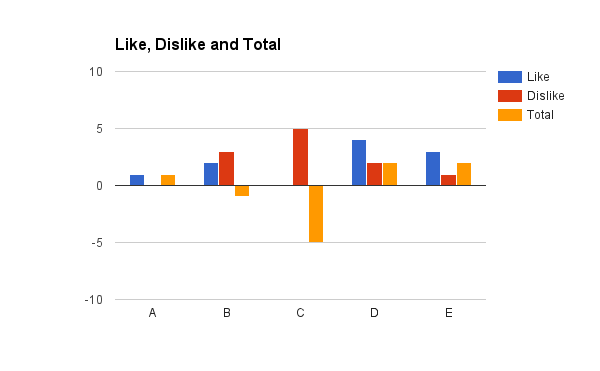
\includegraphics[width=\textwidth]{images/layout_feedback}
	\caption{Column chart showing the number of positive, negative and cumulative votes for each layout.}
	\label{fig:layout_feedback}
\end{figure}

A summary of the most recurring comments about each interface is listed below.

\begin{enumerate}[label=\Alph*,topsep=0pt]
	\item 
	\begin{itemize} 
		\item[+] The interface is simple and clear. 
		\item[-] It is not descriptive enough, it is hard to know what each element corresponds to.
	\end{itemize}
	
	\item 
	\begin{itemize}
		\item[+] All the elements are visible on the screen without asking any effort to understand them.
		\item[-] The lack of images makes the interface less attractive.
	\end{itemize} 
	
	\item
	\begin{itemize}
		\item[+] Everything is kept together, on one screen.
		\item[-] The amount of information on the screen is too large, therefore there will be too much scrolling involved.
	\end{itemize} 
	
	\item
	\begin{itemize}
		\item[+] The accordion makes the navigation smoother: it keeps a good overview of all the information that has to be input, while giving the impression that the amount of input is not too big. It also keeps everything on the same screen, but does not require too much scrolling.
		\item[-] The interface seems more complex, therefore less engaging. Moreover, it is slightly harder to see what is going on and what to do.
	\end{itemize} 
	
	\item
	\begin{itemize}
		\item[+] The simplicity and clarity of the design makes it more engaging: there is less information on the screen, which makes it easier to focus on one thing at a time.
		\item[-] The fact that it is necessary to press a button to move from one step to another makes the whole process too long.
	\end{itemize} 
\end{enumerate}

\subsection*{Selectors}

\Cref{fig:selector_feedback} shows the number of votes each feature input type received, with the same format as \Cref{fig:layout_feedback}. 

\begin{figure}[h]
	\centering
	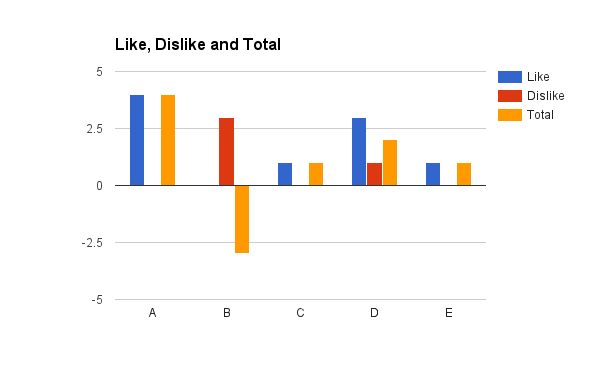
\includegraphics[width=\textwidth]{images/selector_feedback}
	\caption{Column chart showing the number of positive, negative and cumulative votes for each feature selector.}
	\label{fig:selector_feedback}
\end{figure}

Again, a summary of the most recurring comments about each interface is listed below.

\begin{enumerate}[label=\Alph*,topsep=0pt]
	\item 
	\begin{itemize}
		\item[+] The images and the slot machine make the interface attractive and fun to use.
		\item[-] Although one user enjoyed the idea of having to guess which feature had to be input, based only on the image, most participants would prefer to have captions below the images.
	\end{itemize}
	
	\item 
	\begin{itemize}
		\item[-] Most participants either did not say anything about this attribute selection type, or mentioned that they did not like the lack of images, because it did not catch their attention.
	\end{itemize} 
	
	\item
	\begin{itemize}
		\item[+] One participant liked the basic idea of going through the images horizontally, but suggested the use of swiping cards rather than scrollable areas.
		\item[-] Similarly to interface B, most participants did not have anything to say about this selector. Two of them reiterated their dislike of scrollbars.
	\end{itemize} 
	
	\item
	\begin{itemize}
		\item[+] A few participants enjoyed the carousel because if shows several options in the same view. They suggested that it showed a preview of the other images, as well as the currently displayed one. 
	\end{itemize} 
	
	\item
	\begin{itemize}
		\item[+] One participant liked this selector because it allowed the users to see multiple images at the same time.
		\item[-] This time again, most participants did not have any particularly strong view about this last selector, other than the scrolling involved, which they dislike.
	\end{itemize} 
\end{enumerate}

\begin{figure}
	\centering
	\begin{subfigure}{0.3\textwidth}
		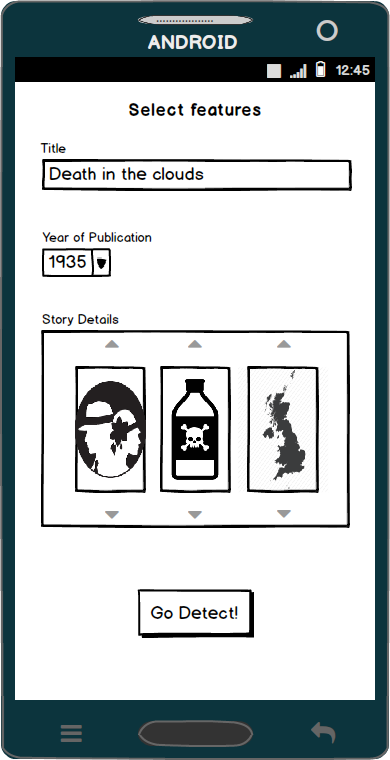
\includegraphics[width=\textwidth]{images/single_fruit_machine}
		\caption{Wireframe A.}
		\label{fig:wireframeA}		
	\end{subfigure}
	\quad
	\begin{subfigure}{0.3\textwidth}
		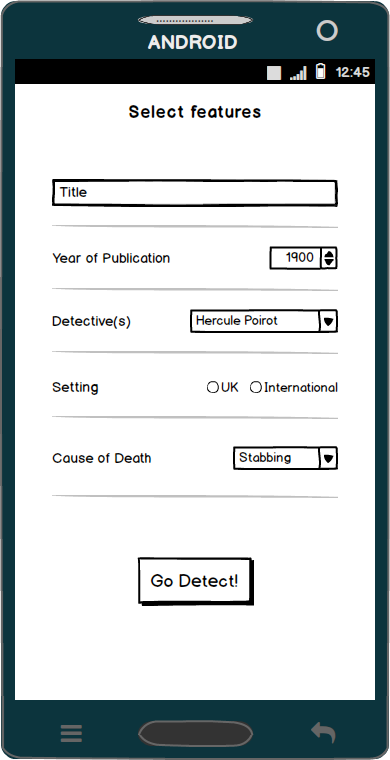
\includegraphics[width=\textwidth]{images/single_text_only}
		\caption{Wireframe B.}
		\label{fig:wireframeB}		
	\end{subfigure}
	
	\begin{subfigure}{\textwidth}
		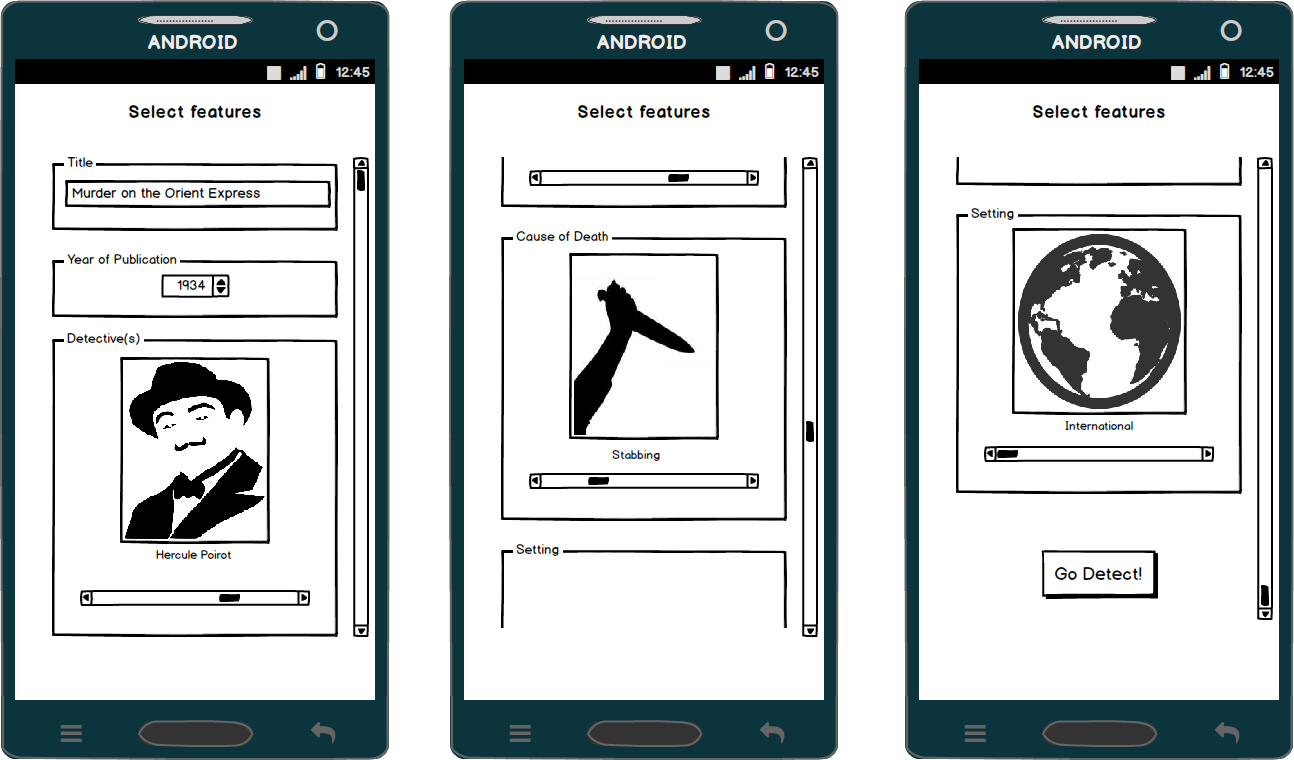
\includegraphics[width=\textwidth]{images/single_list}
		\caption{Wireframe C.}
		\label{fig:wireframeC}		
	\end{subfigure}
	\caption{Wireframes A, B and C.}
\end{figure}

\begin{figure}
	\centering
	
	\begin{subfigure}{\textwidth}
		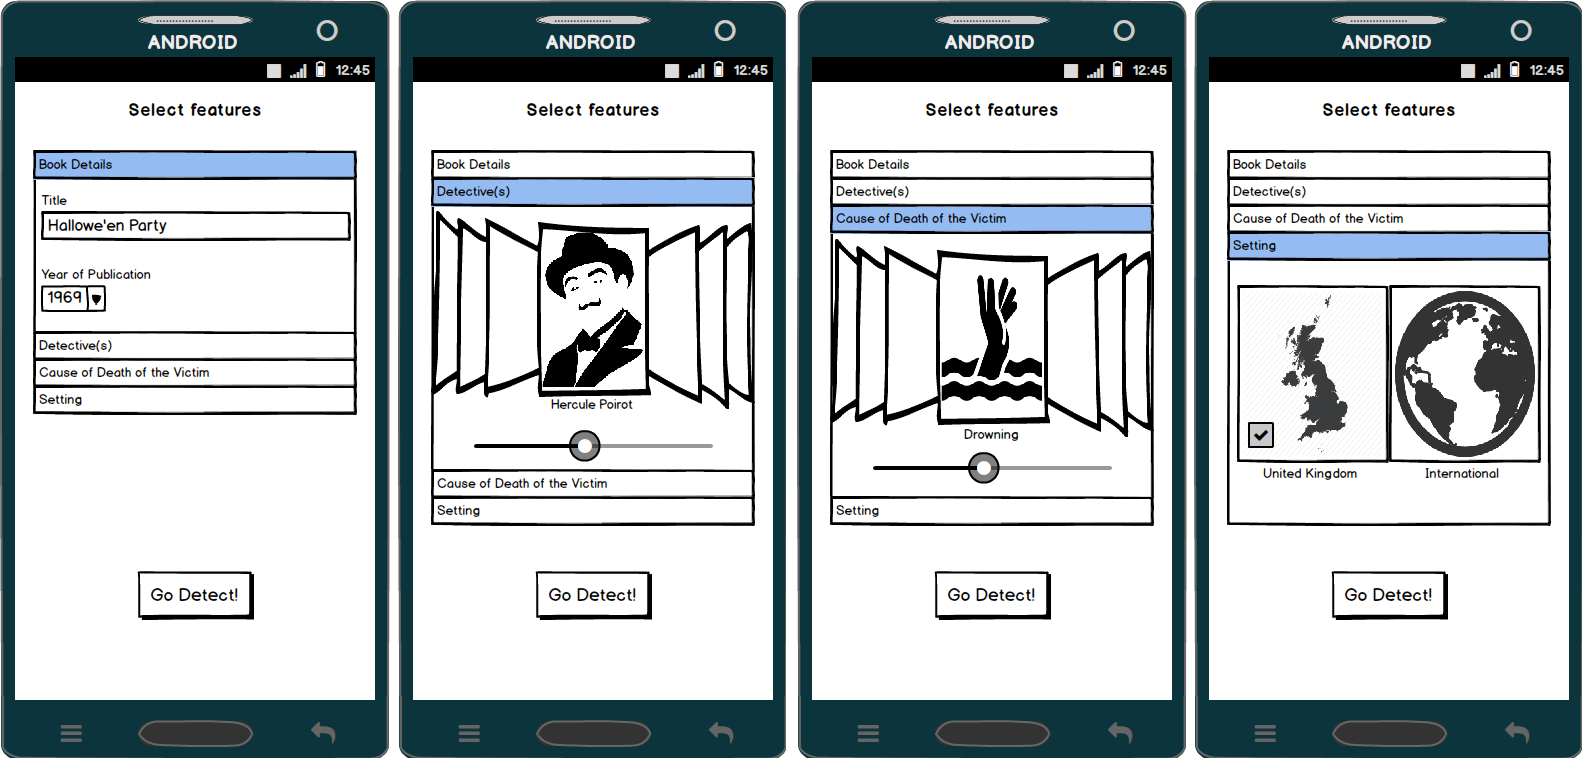
\includegraphics[width=\textwidth]{images/single_accordion}
		\caption{Wireframe D.}
		\label{fig:wireframeD}		
	\end{subfigure}		
	
	\begin{subfigure}{\textwidth}
		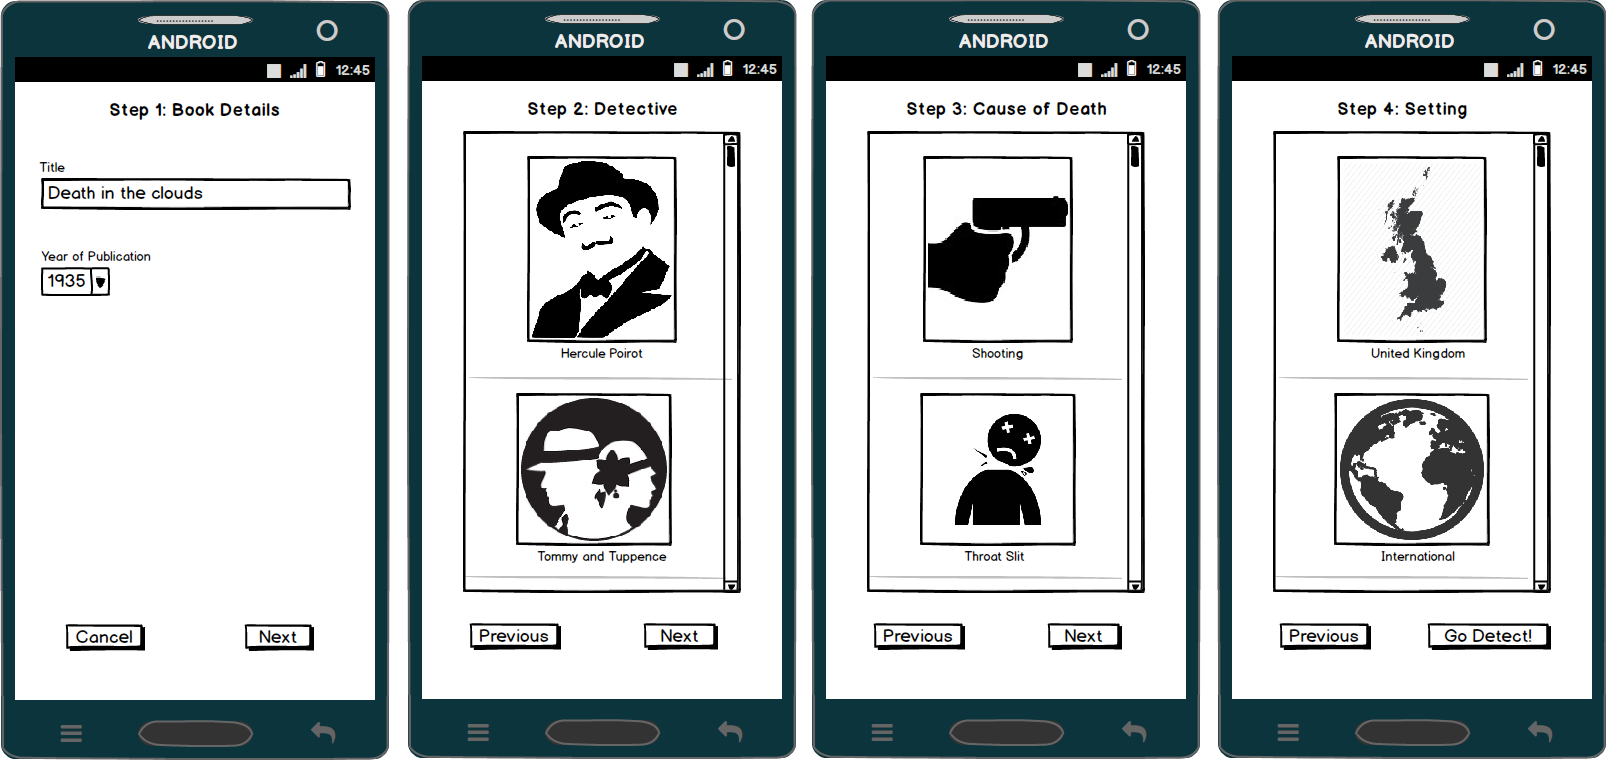
\includegraphics[width=\textwidth]{images/multiple_list}
		\caption{Wireframe E.}
		\label{fig:wireframeE}		
	\end{subfigure}			
	\caption{Wireframes D and E.}
\end{figure}


%%%%%%%%%%%%%%%%%%%%%%%%%%%%%%%%%%%%%%%%%%%%%%%%%%%%%%%%%%%%%%%%%%%
\chapter{Implementation}\label{implementation}

The implementation section of the project was divided into three iterations. 
The first iteration aimed at creating a fixed predictor: the user inputs data, and receives a prediction (user stories 1, 2 and 5). 
The objective of second iteration was to retrain the classifier on the app (user stories 6 and 7). 
For the last iteration, crowdsourced data gathering and training were implemented (user stories 8 and 9). \par

%%%%%%%%%%%%%%%%%%%%%%%%%%%%%%%%%%%%%
\section{Technologies Used}

\subsection{Scrapy}\label{scrapy}

Scrapy is an application framework written in Python, which can be used to extract data from Web sites \cite{scrapy}, created by Scrapinghub's co-founders Pablo Hoffman and Shane Evans. \cite{scrapinghub}

Scrapy is free and open source. It also provides a lot of support, as it comes with a tutorial in addition to a detailed documentation. \cite{scrapydoc}

\subsubsection*{Difficulties Encountered}

Scrapy was not hard to learn or use, thanks to the documentation. It was used in conjunction with the Goodreads API \cite{goodreadsapi} to extract the number of ratings and the ratings average for each novel in the training set. The main and only problem with the web scraping process was faced because the books were searched using their titles only, which resulted in a few instances assigned to the data of a novel with the same title, but a different author. I therefore verified the extracted values ``by hand'', by comparing them to the data visible on the Agatha Christie's books page. \cite{goodreads}

%%%%%%%%%%%%%%%%%%%%%%%%%%%%%%%%%%%%%
\subsection{Android}

The mobile application was implemented using Android, which is an open source operating system for mobile devices (smartphones and tablets), developed by Google and released in 2008.\cite{androidrelease} The phone used for this project is a Samsung Galaxy S3 LTE, running on Android 4.4.4 (KitKat platform).

It was chosen because I became familiar with Java during the past couple of years, as it is the main programming language used in the Masters courses. It was also an occasion for me to get some experience in Android development, which I was interested in. In addition, Android is the most used mobile operating system worldwide. \cite{androidsales} Furthermore, the Android SDK offers a lot of flexibility, as it can be downloaded on Windows, Mac OS, or Linux, and used with the Android's free IDE Android Studio. \cite{androidstudio} Lastly, there is a vast amount of documentation and tutorials available for developing with the Android SDK. \cite{androidtutorials} \cite{thebignerdranchguide}

\subsubsection*{Difficulties Encountered}

Creating the Android interface itself was not particularly hard. It did require a significant amount of time to browse through all the widgets available in the different Android standard libraries (seven Android packages contain widgets \cite{androidpackages}), then to decide which ones were the most appropriate for the app, and to learn how to customise and control them programmatically. Compatibility was also an issue, for some UI elements or attributes were introduced in more recent Android versions than the app's target version. It was therefore necessary to find alternative solutions. \par

However, none of those obstacles were a surprise; as a matter of fact, they are an integral part of the learning process, and overcoming such difficulties can only have a positive impact on my overall programming experience. \par

The hardest part of the Android development was to try to make the app as reliable and efficient as possible. This includes facing all the possible causes for the app to crash unexpectedly, which involves handling the activity lifecycle of the app \cite{androidlifecycle} (what to do when the app is paused, resumed, stopped), properly managing the different activities and fragments, as well as the way they communicate. It also includes monitoring the amount of memory and battery use of the app.
Unfortunately, although this was one of the main points of concern, not all of these elements were fully handled. \par

Another difficulty arose on a code-level, when trying to reduce the amount of redundancy from one activity or fragment to another, without making the overall code harder to read. Because of the way projects are structured in Android \cite{androidprojects}, it is necessary to jump from one file to another in order to follow the flow of the system. This becomes worse when creating extra classes to store the common code shared by multiple elements.

%%%%%%%%%%%%%%%%%%%%%%%%%%%%%%%%%%%%%
\subsection{Weka}

To make predictions, this app referenced machine learning algorithms implemented in the Weka workbench \cite{weka}, created by Eibe Frank, Mark Hall, Peter Reutemann, and Len Trigg.

This is the machine learning library used for the project because it is written in Java, which means it should be possible to use it with an Android application. It is also open source, and is documented in a book about Data Mining and Machine Learning, written by some of the Weka developers. \cite{wekabook}

\subsubsection*{Difficulties Encountered}\label{wekadiff}

As mentioned previously, the machine learning side of this project was handled using the Weka package. Thus, a large part of the time was spent researching the different functionalities available in the Weka explorer \cite{wekaexplorer}, and understanding how to programmatically get the same information as the one produced using the GUI. As a result, a utility class was created, containing methods to create instances (from user input or from a file), to filter those instances, to create a classifier and train it on the instances, to evaluate the classifier, to classify one or more instances and retrain the classifier on new data. \par

This preliminary work was difficult, mainly because it was hard to find explanations in the documentation, for the different exceptions that were thrown when executing some instructions. The exception messages were not descriptive enough, and it took a lot of reading of problems faced by other users of the library to eventually find the causes of the errors. \par

Merging the functionalities implemented in the utility class with the Android code happened without almost any obstacle. The .jar file containing the source code of the library was added as a dependency in the project, and all the needed classes were imported in the standard way\footnote{``\texttt{import weka.}'' followed by the package containing the class to be used, and the name of the class.}. The only encountered issue came from the fact that, in order to train a classifier, one of the Weka classes uses the Java \verb|GraphicsEnvironment class| from the \verb|awt| package\footnote{http://grepcode.com/file/repo1.maven.org/maven2/org.pentaho.pentaho-commons/pentaho-package-manager/1.0.8/org/pentaho/packageManagement/PackageManager.java\#PackageManager.setProxyAuthentication\%28java.net.URL\%29}, which is not available in Android. It was therefore not possible to train the classifier on the app. This was fixed by training it externally, outputting the trained object to a .model file, including that file as an asset of the project (as described previously in \Cref{data_process}), and recreating the corresponding Classifier object from the .model file when launching the app.

%%%%%%%%%%%%%%%%%%%%%%%%%%%%%%%%%%%%%
\subsection{Django \& Heroku}

\subsubsection*{Django}

Django is a Web application framework written in Python \cite{django}. It facilitates Web development, by providing ``high-level abstractions of common patterns, shortcuts for frequent programming tasks, and clear conventions for how to solve problems.'' \cite{djangobook}

Choosing Django was mainly due to the fact that I had used it for a project in one of the Masters courses. It also has the advantage of being well documented and having an active user community.\par

\subsubsection*{Heroku}

Heroku is a cloud platform which allows users to deploy Web applications and their databases. It aims at speeding up the development process by handling the server management, the deployment and the scaling of the applications. \cite{heroku}

Heroku is free for low traffic sites, it is easy to scale and allows to easily create a PostgreSQL database. It is also possible to link the deployed application to a Github repository, such that any pushed change is automatically applied to the Heroku application. \cite[Chapter~1]{herokubook}

\subsubsection*{Difficulties Encountered}

Using Django did not cause any particular problem. Deploying the app once developed was, however, trickier than expected when following the official documentation only. I was getting confused about all the different components that had to be installed, and how they all related to one another. It was however easier to understand the process, using the Django Girls tutorial. \cite{djangogirls}

%%%%%%%%%%%%%%%%%%%%%%%%%%%%%%%%%%%%%
\subsection*{Updated System Architecture}

The following \Cref{fig:architecture_updated} shows the system's architecture with updated labels according to the technologies used for the different components.

\begin{figure}[h]
	\centering
	\includegraphics[width=\textwidth]{images/system_architecture_updated}
	\caption{System's Three-Tiered Architecture.}
	\label{fig:architecture_updated}
\end{figure}

%%%%%%%%%%%%%%%%%%%%%%%%%%%%%%%%%%%%%
\section{Machine Learning Algorithm}

Weka contains over 50 implementations of classifiers. \cite[Table~11.5]{wekabook} However, only 10 of them can be updated without having to retrain them completely (which, as mentioned in previous \Cref{wekadiff}, cannot be done on Android), implementing the \verb|UpdateableClassifier| interface. \cite{wekaupdateable} 7 of these classifiers were applied on the training set : \Cref{tab:updateable} shows the percentages of correctly classified instances of the training set, using those classifiers, when predicting the cause of death of the victim, and the gender of the murderer. The 3 missing classifiers were not used because they either only handle numeric attributes (\verb|NaiveBayesMultinomialUpdateable|), string attributes (\verb|SGDText|) or binary classes (\verb|SGD|).

\begin{table}[h]
	\centering
	\caption{Percentages of correctly classified instances of the initial dataset, for the victim's cause of death and the murderer's gender, using Updateable Classifiers, after training.}
	\begin{tabular}{ |l|c|c| }
		\hline
		\textbf{Classifier}            & \textbf{Cause of death} 					 & \textbf{Murderer's gender} 					  \\
		\hline		
		HoeffdingTree                  & 37                                          & 58                                             \\
		\textbf{IBk}                   & \textbf{100}                                & \textbf{100}                                   \\
		\textbf{KStar}                 & \textbf{100}                                & \textbf{100}                                   \\
		LWL                            & 46                                          & 73                                             \\
		MultiClassClassifierUpdateable & 48                                          & 73                                             \\
		NaiveBayesMultinomialText      & 37                                          & 58                                             \\
		NaiveBayesUpdateable           & 42                                          & 60                                             \\
		\hline
	\end{tabular}
	\label{tab:updateable}
\end{table}

The two most accurate classifiers are IBk and KStar. Both algorithms use \textbf{nearest-neighbour classification}, which consists in comparing each new instance to existing ones, by calculating the distance separating the new instance to known instances, and predicts the same class as the training instance which is the closest to the new instance. \cite[Chapter~3]{wekabook} \par 

Since both classifiers seemed to have similar performances, IBk was arbitrarily chosen. IBk looks for the closest training example using the \textbf{Euclidean distance} \cite[Chapter~11]{wekabook}. To compute the distance between two instances $A^{(1)}$ with $k$ attributes $a_1^{(1)}, a_2^{(1)}, ..., a_k^{(1)}$ and $A^{(2)}$ with $k$ attributes $a_1^{(2)}, a_2^{(2)}, ..., a_k^{(2)}$, it is first necessary to define the \textbf{difference between two attributes} $a_i^{(1)}$ and $a_i^{(2)}$. \cite[Chapter~4]{wekabook}

If the attributes are numeric, then the difference between them is 
\begin{center}
	$(a_i^{(1)} - a_i^{(2)})$.
\end{center}

However, numeric attributes have to be normalized, as two different attributes could have different scales (for example, the year of publication is greater than 1800, whereas the average ratings is less or equal to 5). Given $v_i$ the actual value of attribute $i$, $a_i$ becomes:
\begin{center}
	$a_i = \frac{v_i - \text{min } v_i}{\text{max } v_i - \text{min } v_i}$
\end{center}
with min $v_i$ and max $v_i$ being respectively the minimum and the maximum values of attribute $i$ in the entire training set. 

If the attributes are nominal, the difference between them is
\begin{equation}
	\begin{cases}
		0, & \text{if the attributes are the same}\\
		1, & \text{otherwise}\\
	\end{cases}
\end{equation}

The Euclidean distance between two instances $A^{(1)}$ and $A^{(2)}$ is therefore
\begin{center}
	$\sqrt{(a_1^{(1)} - a_1^{(2)})^2 + (a_2^{(1)} - a_2^{(2)})^2 + ... + (a_k^{(1)} - a_k^{(2)})^2}$.
\end{center}

As mentioned in \Cref{data_process}, a new instance of the \verb|IBk| class was created, trained on the initial dataset, using 5-folds \textbf{cross-validation}: this technique consists in splitting the dataset in 5 partitions, and in turn, using each partition for testing the result of training on the other partitions. \cite[Chapter~5]{wekabook} The trained classifier was then output to a .model file, which was stored in the Android project as an asset, so the classifier object could be retreived within the app.

\subsection*{ARFF Files}

Weka requires datasets to be provided in ARFF format (which stands for attribute-relation file format). \cite{arff} ARFF files consist in two parts:
\begin{itemize}[topsep=0pt]
	\item the header, which contains 
	\begin{itemize}
		\item the name of the relation (typically what each instance of the dataset represents --- in our case, ``novel''), preceded by \verb|@RELATION|,
		\item the list of attributes with the following format: \verb|@ATTRIBUTE name type|,
	\end{itemize}
	\item the data, preceded by \verb|@DATA|, with each instance on a different line, and the values for each instance separated by commas.
\end{itemize}

%%%%%%%%%%%%%%%%%%%%%%%%%%%%%%%%%%%%%
\section{Story Details Input}

\subsection*{Customization of the User Interface}

The user experiment described in \Cref{wireframes} showed two main groups of users: those who favoured a clear, simple interface, which did not require much effort to read or understand, and those who enjoyed an interactive interface with images better. Because it did not seem possible to create one interface which could satisfy all the users, several layouts were implemented, so users could customize their own application by changing the settings, as shows figure ....

[Screen shot of settings screen]

\textbf{??} and \textbf{??} show two different interfaces, displaying the same information.

[Screen shots of main activity using text and using images]

Users can also choose to select the concept to be predicted using a pop-up window, or tabs on the main screen, as can be seen on \textbf{??} and \textbf{??}.

[Screen shots of class dialog and class tabs]

Finally, when the ``Story details Input'' is set to ``Images'', users can choose to browse through the images of the attributes they have to input using a spinner (\textbf{??}) or view all of them in a grid (\textbf{??}).

[Screen shots of grid view and spinner view]

%%%%%%%%%%%%%%%%%%%%%%%%%%%%%%%%%%%%%
\subsection*{Attributes Selection}

In order to select the features they want to input, users can press check boxes for all the attributes they are interested in, displayed in a pop-up window (\textbf{??}) or a navigation drawer (\textbf{??}): this is also customizable in the settings.

[Screen shots of dialog and drawer]

As visible on \textbf{??} and \textbf{??}, the number of ratings, extracted from Goodreads, was not included after all, since users cannot know this information about the book they are interested in, unless they are able to access the website themselves, which is not assumed to be true (as the system should be usable off-line). For the same reason, no attempt was made to get the app to fetch the information itself. \par

Furthermore, the title of the novel is ignored by the classifier, and only used to keep track of the novel of interest. The reason for this is that the IBk classifier cannot handle string attributes. It is therefore necessary to filter the title so it is converted into a nominal attribute (using the \verb|StringToNominal| filter) or into a ``set of nominal attributes representing word occurrence information from the text contained in the string'' (using the \verb|StringToWordVector| filter). However, filters cannot be applied to attributes in the app's code because they also use a class from the \verb|java.awt| package, which is, as mentioned in \Cref{wekadiff}, not available in Android.

%%%%%%%%%%%%%%%%%%%%%%%%%%%%%%%%%%%%%
\subsubsection*{Missing Values}
The unselected attributes are handled as missing. In Weka, missing values are treated differently for each classifier. When two attributes $a_i^{(1)}$ and $a_i^{(2)}$are compared with IBk, if one of them (say $a_i^{(1)}$) has a missing value, then:
\begin{itemize}[topsep=0pt]
	\item if it is a numeric attribute, the difference between the attributes is
	\begin{equation}
		\begin{cases}
			1, & \text{if } a_i^{(2)} \text{also has a missing value} \\
			\text{max( }a_i^{(2)} , 1 - a_i^{(2)} \text{)}, & \text{otherwise;} \\
		\end{cases}
	\end{equation}
	\item if it is a nominal attribute, the difference between the attributes is 1.	
\end{itemize}

%%%%%%%%%%%%%%%%%%%%%%%%%%%%%%%%%%%%%
\section{Prediction Output}

Once all the fields corresponding to the selected attributes have been populated, users can press the ``Go Detect'' button, and generate a prediction based on their input (\textbf{??}). 

[Screen shot of prediction activity]

Based on the probability distribution of the predicted value, and on the number of input attributes, the prediction is followed by a sentence simulating the system expressing how confident it is about its guess (this seemed more user-friendly than simply outputting a percentage).\par

Users can then press
\begin{itemize}[topsep=0pt]
	\item ``Back'' to return to verify or rectify their input,
	\item the ``Correct'' button to validate the prediction, and go back to the reset details input screen,
	\item the ``Incorrect'' button and be prompted to submit the value that should have been predicted.
\end{itemize}

[Screen shots of dialogs]

%%%%%%%%%%%%%%%%%%%%%%%%%%%%%%%%%%%%%
\section{Communication with the Server}

In the earliest version of the system during the third iteration, the training dataset was stored on the server-side, in a .txt file which could be downloaded by the clients, or updated by the server when new data was added. \par

When a user launched the app, it had to check whether new entries were added since the last time the app was used. The initial way to do this was to compare the size of the two files: if the server's file was larger than the local one, it meant that the app's dataset had to be updated. This did not work as expected however, because when an application is deployed on Heroku, it is assembled into a compressed bundle \cite{herokuslug}. Consequently, the size of the file stored on the server was not accurate. \par 

To overcome this issue, the number of entries in the dataset was stored in a database. This integer was incremented for every new instance shared by a user, and used instead to compare the two datasets. If the app's training set had fewer instances, it would then download the content of the server's file, extract the newest entries, and update the classifier on each entry, while also adding it to the local file. When a user invalidated a prediction and agreed to share the details with the other users, the data was sent as a string to the server, which added a new line to the file with that data.\par

This was easy and convenient, especially for testing, but not optimal in terms of scalability: if several thousands of users were to use the app, and the training set updated regularly, that file would quickly become very large, and having all the users to download it every time they launch the app would not be practical. Alternatively, all the instances of server's training set were stored in the database. Instead of downloading the whole content of a file, the client-apps now only fetch the new entries when the user starts the app. This is described in \Cref{fig:launch}.
\begin{figure}[h]
	\centering
	\includegraphics[width=\textwidth]{images/app_launching_diagram}
	\caption{Sequence diagram showing the communication within the system when the user launches the app.}
	\label{fig:launch}
\end{figure}

In order to check whether an entry is new to a given client, each entry is assigned a timestamp with the date and time it was sent to the server. Each client also keeps the time it last downloaded new data, so that the server can send all the entries that were added after the client's last update. Additionally, when the user submits new data, a new entry is created in the database, and the server returns the timestamp for the transaction, as shown in \Cref{fig:new_entry}.
\begin{figure}[h]
	\centering
	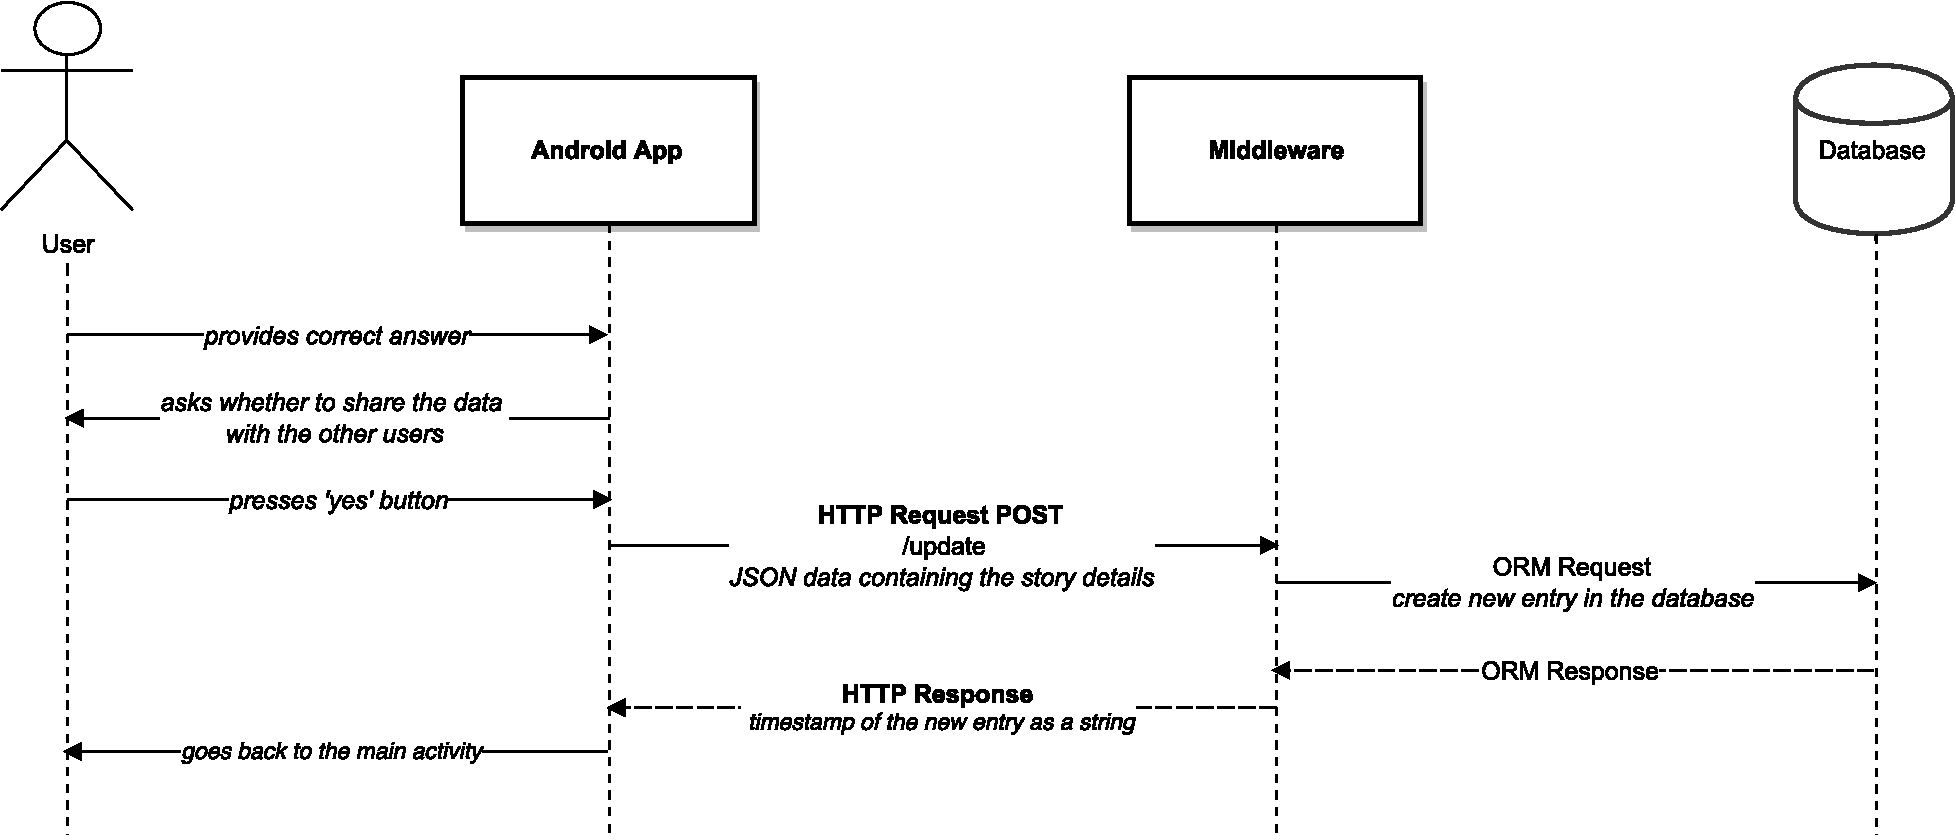
\includegraphics[width=\textwidth]{images/wrong_prediction_diagram}
	\caption{Sequence diagram showing the communication within the system when the user invalidates a prediction.}
	\label{fig:new_entry}
\end{figure}

%%%%%%%%%%%%%%%%%%%%%%%%%%%%%%%%%%%%%
\section{Testing}

(Testing)

%%%%%%%%%%%%%%%%%%%%%%%%%%%%%%%%%%%%%%%%%%%%%%%%%%%%%%%%%%%%%%%%%%%
\chapter{Evaluation}\label{evaluation}

Two evaluation sessions were organised one on the wireframes, and one on the final application. 



%%%%%%%%%%%%%%%%%%%%%%%%%%%%%%%%%%%%%
\section{Final App}

For the final product evaluation,  were first asked to list the possible attributes (year of publication, point of view, location, detective, murder weapon, victim's gender, murderer's gender and ratings) in a random order. They were then given access to the training set, and were asked to pick 5 different titles from the dataset. \par

Based on the order in which they had listed the features, they were had to produce predictions for each one of the 5 novels they picked, leaving out between 0 and 5 attributes. The idea was to show them that the instances were selected randomly, so that, in case they received the right answers, it did not look like I had chosen novels for which I knew the predictions would be correct. They were also given the choice to use any other novel, as long as they were certain of the correctness of the details of the story, which would impact the accuracy of the predictions. \par 

Once the prediction was obtained, they had to decide whether or not to retrain the classifier or to send data to the server. They were also required to modify the settings of the app (related to the interface and the data sharing) after each prediction. \par

For the last part of the evaluation, they were given the possibility to play with the system as they wished.\par

During the whole process, I observed the participants while they used the system, and recorded the time it took them to execute the tasks. I also used the Concurrent Think Aloud method \cite{usabilitytest} which consisted in encouraging them to comment on their actions, taking notes of their observations.


%%%%%%%%%%%%%%%%%%%%%%%%%%%%%%%%%%%%%%%%%%%%%%%%%%%%%%%%%%%%%%%%%%%
\chapter{Conclusion}\label{conclusion}

\section{Summary}

\section{Limitations and Future Work}

\subsection*{Additional functionalities}

\hspace{5mm} Mostly due to a lack of time, two functionalities were not implemented.\par

The first one corresponds to the user stories number 3 and 4 mentioned in the Requirements section, to allow the users to make a guess on the identity of the killer, and receive the likelihood of their supposition to be correct. The users would have to input details about the character they suspect, and the app would compare those elements to its own prediction. Based on the number of matching attributes, the app could output a percentage notifying the users how close they are of finding the culprit. \par

Another potential functionality is related to the context of the user-interaction with the system. The idea is for detective novels fans to be able to use the app, while reading a book. If they get a clue on the murderer before the end of the story, they cannot know whether or not the prediction is right, as the identity of the culprit has not been revealed yet. It could therefore be made possible for the users to save the prediction they received, and go back to it later to confirm it or input the correct data if it was wrong.

\subsection*{Accuracy}

The accuracy of the predictions could be increased by improving the dataset, so that the algorithm can handle much more details about the story. It would therefore be necessary to try and find extra attributes that have an impact on the prediction. Such additional features could be the profession of the murderer, the relationship between the murderer and the victim or the chapter in which the murderer is first introduced. \par

Once such attributes were found, the interface of the app could then be updated, so that it can handle more concepts, other than the murder weapon and the gender of the murderer. Thus any attribute directly related to the murderer could be the possible target of the predictions.
It could also be useful to consider features related to the title of the book: for example checking if the title contains a reference to a location, to a person, to a mean of transport, or to a weapon, and whether such reference helps to infer anything about the murderer.
	
\subsection*{Scalability}

In order to reduce the time spent waiting for the different components to exchange information, in the event of having several thousands of users, the system could be to remodelled, so that the training is handled by the server and not the client. The server would not even need to store any data, it would just receive it, retrain the classifier, and send a .model file containing the output classifier, which could then be loaded by the client to retrieve the Classifier object. \par

This solution would then require using the Weka library with python, which is only possible to a certain extent, given that none of the different packages and libraries which can be used for this purpose seems to implement all the functionalities found in the Java version of Weka \cite{wekapython}. It might even be necessary to use a completely different library, to be exclusively used with Python, such as scikit-learn \cite{scikit-learn} or pybrain \cite{pybrain}. \par

Another approach could be to handle all the machine learning side of the system on the server: the mobile app would just serve as an interface for the users to input data and view the predictions, but the data would be sent to and processed on the server, which would take care of the training, the classification, and the classifier update (as described for the second solution). \par

This solution has several advantages. The first one is that it reduces the client-server communications to the minimum, that is, when the users request a prediction, and when they submit the correct answer after the system made a wrong conjecture. The data sent in those cases would be up to a few hundreds of bytes, which means that the requests would be sent in a few seconds at most. \par

Another advantage is that the Android app would not have to store the .jar file containing the Weka source code, or any of the classes which handle the machine learning, and would therefore take much less space in the devices' memory. It would also use less memory, given that it would have fewer processes to handle. \par

Moreover, it would substantially increase the reusability and portability of the system. Indeed, this structure would allow a better separation of concerns, making the system responsible for the backend, and the device for the frontend. As a result, it would be much easier for another developer to implement the system for other Operating Systems, by only having to modify the code for the interface. \par

The drawbacks, however, include the restriction caused by using Weka in Python, as well as enforcing the users' devices to be connected to the network for the app to output any prediction. This is not the case with the current version, as the users are asked permission before downloading the updated dataset, or before sending the correct answer to the server. Should they choose to refuse, they would miss out on additional data to make the predictions more accurate, yet their classifier would still be locally updated.

\section{Reflection on the Project}

%%%%%%%%%%%%%%%%%%%%%%%%%%%%%%%%%%%%%%%%%%%%%%%%%%%%%%%%%%%%%%%%%%%

\bibliographystyle{apalike}
\bibliography{mproj}

%%%%%%%%%%%%%%%%%%%%%%%%%%%%%%%%%%%%%%%%%%%%%%%%%%%%%%%%%%%%%%%%%%%
\appendix

%%%%%%%%%%%%%%%%%%%%%%%%%%%%%%%%%%%%%%%%%%%%%%%%%%%%%%%%%%%%%%%%%%%

\chapter{Training Set}\label{dataset}

\% 1. Title: Agatha Christie Novels\\
\% 2. Sources:\\
\%\hspace{5mm}(a) Creator: Jeremy Singer \& Clemence Brival\\
\%\hspace{5mm}(b) Date: July, 2016\\
@relation novel

@attribute title string\\
@attribute year numeric\\
@attribute detective \{unknown, `Tommy and Tuppence', `Hercule Poirot', `Colonel Race', `Superintendent Battle', `Miss Marple', `Mystery novel'\}\\
@attribute location \{unknown, UK, International\}\\
@attribute point\_of\_view \{unknown, Third, First\}\\
@attribute murder\_weapon \{unknown, Poison, Stabbing, Accident, Shooting, Strangling, Concussion, ThroatSlit, Drowning, None\}\\
@attribute average\_ratings numeric\\
@attribute number\_of\_ratings numeric\\
@attribute victim\_gender \{unknown, F, M, None\}\\
@attribute murderer\_gender \{unknown, F, M, Lots, None\}

@data\\
`The Mysterious Affair at Styles',1920,`Hercule Poirot',UK,First,Poison,3.96,122922,F,M\\
`The Secret Adversary',1922,`Tommy and Tuppence',UK,Third,Poison,3.82,22649,F,M\\
`The Murder on the Links',1923,`Hercule Poirot',International,First,Stabbing,3.77,18910,M,F\\
`The Man in the Brown Suit',1924,`Colonel Race',International,First,Accident,3.95,49495,M,M\\
`The Secret of Chimneys',1925,`Superintendent Battle',UK,Third,Shooting,3.83,8651,M,F\\
`The Murder of Roger Ackroyd',1926,`Hercule Poirot',UK,First,Stabbing,4.17,66801,M,M\\
`The Big Four',1927,`Hercule Poirot',UK,First,Poison,3.61,17901,M,M\\
`The Mystery of the Blue Train',1928,`Hercule Poirot',International,Third,Strangling,3.75,17262,F,M\\
`The Seven Dials Mystery',1929,`Superintendent Battle',UK,Third,Poison,3.78,9968,M,M\\
`The Murder at the Vicarage',1930,`Miss Marple',UK,First,Shooting,4.02,85677,M,F\\
`The Sittaford Mystery',1931,`Mystery novel',UK,Third,Concussion,3.67,7240,M,M\\
`Peril at End House',1932,`Hercule Poirot',UK,First,Shooting,3.87,18613,F,F\\
`Lord Edgware Dies',1933,`Hercule Poirot',UK,First,Stabbing,3.87,15536,M,F\\
`Why Didn't They Ask Evans?',1934,`Mystery novel',UK,Third,Accident,3.83,11190,M,M\\
`Murder on the Orient Express',1934,`Hercule Poirot',International,Third,Stabbing,4.13,136560,M,Lots\\
`Three Act Tragedy',1935,`Hercule Poirot',UK,Third,Poison,3.8,10616,M,M\\
`Death in the Clouds',1935,`Hercule Poirot',UK,Third,Poison,3.77,17294,F,M\\
`The A.B.C. Murders',1936,`Hercule Poirot',UK,First,Concussion,3.95,47222,F,M\\
`Cards on the Table',1936,`Hercule Poirot',UK,Third,Stabbing,3.88,19266,M,M\\
`Murder in Mesopotamia',1936,`Hercule Poirot',International,First,Concussion,3.84,20756,F,M\\
`Death on the Nile',1937,`Hercule Poirot',International,Third,Shooting,4.04,62803,F,M\\
`Dumb Witness',1937,`Hercule Poirot',UK,First,Poison,3.79,11233,F,F\\
`Appointment with Death',1938,`Hercule Poirot',International,Third,Poison,3.83,20383,F,F\\
`Hercule Poirot\'s Christmas',1938,`Hercule Poirot',UK,Third,ThroatSlit,3.88,18770,M,M\\
`Murder Is Easy',1939,`Superintendent Battle',UK,Third,Accident,3.74,9034,F,F\\
`And then there were none',1940,`Mystery novel',UK,Third,Poison,4.21,364542,M,M\\
`One Two Buckle My Shoe',1940,`Hercule Poirot',UK,Third,Shooting,3.72,12553,M,M\\
`Sad Cypress',1940,`Hercule Poirot',UK,Third,Poison,3.81,12699,F,F\\
`Evil Under the Sun',1941,`Hercule Poirot',UK,Third,Strangling,3.93,27508,F,M\\
`N or M?',1941,`Tommy and Tuppence',UK,Third,Accident,3.72,11396,M,M\\
`The Body in the Library',1942,`Miss Marple',UK,Third,Poison,3.83,35267,F,F\\
`The Moving Finger',1942,`Miss Marple',UK,First,Poison,3.83,15301,F,M\\
`Five Little Pigs',1942,`Hercule Poirot',UK,Third,Poison,3.93,20068,M,F\\
`Towards Zero',1944,`Superintendent Battle',UK,Third,Concussion,3.83,7921,M,M\\
`Death Comes as the End',1945,`Mystery novel',International,Third,Accident,3.83,9681,F,M\\
`Sparkling Cyanide',1945,`Colonel Race',UK,Third,Poison,3.83,10141,M,F\\
`The Hollow',1946,`Hercule Poirot',UK,Third,Shooting,3.75,17390,M,F\\
`Taken at the Flood',1948,`Hercule Poirot',UK,Third,Concussion,3.69,7706,M,M\\
`Crooked House',1949,`Mystery novel',UK,First,Poison,3.95,15973,M,F\\
`A Murder Is Announced',1950,`Miss Marple',UK,Third,Shooting,3.94,25476,M,F\\
`They Came to Baghdad',1951,`Mystery novel',International,Third,Stabbing,3.77,8935,M,M\\
`They Do It with Mirrors',1952,`Miss Marple',UK,Third,Shooting,3.73,13628,M,M\\
`Mrs McGinty\'s Dead',1952,`Hercule Poirot',UK,Third,Concussion,3.79,11223,F,M\\
`After the Funeral',1953,`Hercule Poirot',UK,Third,Concussion,3.82,13957,F,F\\
`A Pocket Full of Rye',1953,`Miss Marple',UK,Third,Poison,3.82,17224,M,M\\
`Destination Unknown',1954,`Mystery novel',International,Third,Poison,3.64,5096,F,M\\
`Hickory Dickory Dock',1955,`Hercule Poirot',UK,Third,Poison,3.73,11438,F,M\\
`Dead Man\'s Folly',1956,`Hercule Poirot',UK,Third,Strangling,3.76,10723,F,F\\
`4.50 from Paddington',1957,`Miss Marple',UK,Third,Strangling,3.91,24564,F,M\\
`Ordeal by Innocence',1958,`Mystery novel',UK,Third,Concussion,3.76,6680,F,F\\
`Cat Among the Pigeons',1959,`Hercule Poirot',UK,Third,Shooting,3.81,17246,F,F\\
`The Pale Horse',1961,`Mystery novel',UK,First,Poison,3.73,7917,F,M\\
`The Mirror Crack\'d from Side to Side',1962,`Miss Marple',UK,Third,Poison,3.87,19898,F,F\\
`The Clocks',1963,`Hercule Poirot',UK,First,Stabbing,3.69,12905,M,M\\
`A Caribbean Mystery',1964,`Miss Marple',International,Third,Poison,3.76,14663,M,M\\
`At Bertram\'s Hotel',1965,`Miss Marple',UK,Third,Shooting,3.69,14716,M,F\\
`Third Girl',1966,`Hercule Poirot',UK,Third,Accident,3.59,11464,F,F\\
`Endless Night',1967,`Mystery novel',UK,First,Accident,3.74,9748,F,M\\
`By the Pricking of My Thumbs',1968,`Tommy and Tuppence',UK,Third,Poison,3.7,8488,F,F\\
`Hallowe\'en Party',1969,`Hercule Poirot',UK,Third,Drowning,3.66,15341,F,F\\
`Passenger to Frankfurt',1970,`Mystery novel',International,Third,None,3.05,5140,None,None\\
Nemesis,1971,`Miss Marple',UK,Third,Poison,3.74,10439,F,F\\
`Elephants Can Remember',1972,`Hercule Poirot',UK,Third,Shooting,3.62,15546,F,M\\
`Postern of Fate',1973,`Tommy and Tuppence',UK,Third,Poison,3.26,5358,?,?\\
Curtain,1975,`Hercule Poirot',UK,First,Poison,4.03,19280,M,M\\
`Sleeping Murder',1976,`Miss Marple',UK,Third,Strangling,3.9,16477,F,M\\

%%%%%%%%%%%%%%%%%%%%%%%%%%%%%%%%%%%%%%%%%%%%%%%%%%%%%%%%%%%%%%%%%%%
\chapter{Second appendix}

\end{document}
